\documentclass[11pt,a4paper]{article}

% ============================================================
% Packages
% ============================================================
\usepackage[margin=1in]{geometry}
\usepackage{amsmath,amssymb,bm}
\usepackage{graphicx}
\usepackage{booktabs}
\usepackage{longtable}
\usepackage{array}
\usepackage{xcolor}
\usepackage{hyperref}
\usepackage{enumitem}
\usepackage{float}
\usepackage{tikz}
\usetikzlibrary{arrows.meta,positioning,shapes.geometric}

\hypersetup{
    colorlinks=true,
    linkcolor=blue,
    urlcolor=blue,
    citecolor=blue
}

% ============================================================
% Title
% ============================================================
\title{\textbf{Literature Study Notes on Cycle-Jump Algorithms}\\
\large Li et al. (2025) and Cheng, Hu \& Kirka (2022)}
\author{Pruthvi}
\date{\today}

\begin{document}

\maketitle

\begin{center}
\textbf{Prepared for discussion with Dr. Omar}
\end{center}

\vspace{0.5cm}

\noindent
This document summarizes two recent cycle-jump acceleration papers relevant to cyclic plasticity, fatigue crack propagation, and future UMAT/cycle-jump implementation work.

\begin{enumerate}
    \item Li et al. (2025), \textit{An adaptive cycle jump method for elasto-plastic phase field modeling addressing fatigue crack propagation}, Computer Methods in Applied Mechanics and Engineering, DOI: \href{https://doi.org/10.1016/j.cma.2025.118074}{10.1016/j.cma.2025.118074}.
    \item Cheng, Hu and Kirka (2022), \textit{A cycle-jump acceleration method for the crystal plasticity simulation of high cycle fatigue of the metallic microstructure}.
\end{enumerate}

% ============================================================
\section{Big Picture: Why Cycle Jumping Is Needed}

Cyclic fatigue simulations are expensive because each loading cycle must normally be solved increment by increment. If the number of cycles is large, a direct cycle-by-cycle finite element simulation becomes computationally infeasible.

The basic cycle-jump idea is:

\begin{quote}
Compute a few full cycles, identify the slow cycle-to-cycle evolution of the important state variables, extrapolate those variables over several skipped cycles, and then continue the simulation from the predicted state.
\end{quote}

This is useful because fatigue problems usually contain two time scales:

\begin{itemize}
    \item a \textbf{fast time scale}: loading and unloading inside one cycle,
    \item a \textbf{slow time scale}: gradual evolution of plastic strain, damage, crack length, phase field, internal variables, or microstructural state over many cycles.
\end{itemize}

The cycle-jump algorithm tries to skip only the slow evolution part, while still preserving the important physics.

% ============================================================
\section{Paper 1: Li et al. (2025)}

\subsection{Full Reference}

Li, J., Hu, Y., Ao, N., Miao, H., Zhang, X., Kang, G., and Kan, Q. (2025). \textit{An adaptive cycle jump method for elasto-plastic phase field modeling addressing fatigue crack propagation}. Computer Methods in Applied Mechanics and Engineering, 442, 118074. DOI: \href{https://doi.org/10.1016/j.cma.2025.118074}{10.1016/j.cma.2025.118074}.

% ------------------------------------------------------------
\subsection{Main Idea}

Li et al. develop an adaptive explicit cycle-jump method for phase-field fatigue crack propagation in elasto-plastic materials. The key challenge is that phase-field fracture simulations are already expensive because they need fine mesh near the diffused crack. If fatigue crack growth is then simulated cycle by cycle, the cost becomes very high.

The paper accelerates the simulation by extrapolating selected variables over several cycles. The method is designed not only for elastic materials but also for elasto-plastic materials, where crack-tip plasticity affects the crack growth rate.

The main novelty is:

\begin{itemize}
    \item it updates selected phase-field and plasticity-related variables during cycle jumps,
    \item it introduces an adaptive rule to choose the cycle-jump size,
    \item the adaptive rule is based on the evolution of the phase field,
    \item it is verified for different plasticity models and crack configurations.
\end{itemize}

% ------------------------------------------------------------
\subsection{Why This Paper Matters}

This paper matters for the thesis direction because it connects three topics that are important for cyclic fatigue simulations:

\begin{enumerate}
    \item \textbf{fatigue crack propagation},
    \item \textbf{phase-field fracture},
    \item \textbf{elasto-plastic constitutive behavior}.
\end{enumerate}

It is especially useful because it shows how cycle jumping can be adapted when the material response is not purely elastic. For elasto-plastic fatigue, plastic strain accumulation near the crack tip can strongly affect crack propagation. Therefore, an acceleration method must not simply extrapolate the crack variable; it must also account for plasticity-related variables.

% ------------------------------------------------------------
\subsection{Physical Model}

The body is an elasto-plastic solid containing cracks. The crack is not represented as a sharp discontinuity. Instead, the crack is represented by a scalar phase-field variable.

\begin{table}[H]
\centering
\caption{Physical meaning of the main fields in Li et al.}
\begin{tabular}{lll}
\toprule
Symbol & Name & Meaning \\
\midrule
$\Omega$ & body domain & solid region being simulated \\
$\partial \Omega$ & boundary & external boundary of the body \\
$\bm{u}$ & displacement field & mechanical deformation field \\
$\phi$ & phase field & crack/damage variable \\
$\phi=0$ & intact material & no crack \\
$\phi=1$ & fully cracked material & complete failure \\
$\Gamma$ & crack surface & sharp crack in classical fracture theory \\
$l$ & length scale & controls diffused crack width \\
$G_c$ & critical energy release rate & fracture toughness parameter \\
\bottomrule
\end{tabular}
\end{table}

The phase-field variable $\phi$ spreads the crack over a finite width controlled by $l$. This removes the need for explicit crack-path tracking.

% ------------------------------------------------------------
\subsection{Energy Functional}

The total potential energy contains elastic energy, plastic energy, fracture energy, and external work. The original elasto-plastic phase-field energy is written as:

\begin{equation}
\Psi =
\int_{\Omega}
\left[
 g(\phi)\psi^e(\bm{\varepsilon}^e)
+
 g(\phi)\psi^p(\bm{\varepsilon}^p)
\right] dV
+
\int_{\Omega}
\left[
\frac{G_c}{2l}
\left(
\phi^2 + l^2|\nabla \phi|^2
\right)
\right] dV
-
\int_{\Omega}\bm{b}\cdot \bm{u}\,dV
-
\int_{\partial \Omega}\bm{t}\cdot \bm{u}\,dS .
\end{equation}

Here:

\begin{table}[H]
\centering
\caption{Meaning of variables in the energy functional.}
\begin{tabular}{lll}
\toprule
Symbol & Meaning & Comment \\
\midrule
$\Psi$ & total potential energy & minimized by the solution \\
$\psi^e$ & elastic strain energy density & intact material elastic energy \\
$\psi^p$ & plastic strain energy density & plastic work contribution \\
$\bm{\varepsilon}^e$ & elastic strain tensor & recoverable strain part \\
$\bm{\varepsilon}^p$ & plastic strain tensor & irreversible strain part \\
$g(\phi)$ & degradation function & reduces stiffness due to damage \\
$\bm{b}$ & body force & volume force \\
$\bm{t}$ & boundary traction & surface force \\
\bottomrule
\end{tabular}
\end{table}

The degradation function is:

\begin{equation}
g(\phi) = (1-\phi)^2 + \kappa ,
\end{equation}

where $\kappa$ is a small numerical parameter used to avoid singularity when the material is almost fully cracked.

% ------------------------------------------------------------
\subsection{Elastic Energy Split}

The tensile and compressive parts of elastic energy are split as:

\begin{equation}
\psi_e^{\pm}
=
\frac{1}{2}\lambda \langle \text{tr}(\bm{\varepsilon}^e) \rangle_{\pm}^2
+
\mu \text{tr}
\left[
(\bm{\varepsilon}_e^{\pm})^2
\right].
\end{equation}

Here:

\begin{itemize}
    \item $\lambda$ and $\mu$ are Lam\'e constants,
    \item $\langle x \rangle_{\pm} = (x \pm |x|)/2$ is the Macaulay bracket,
    \item the split prevents compression from driving crack growth.
\end{itemize}

% ------------------------------------------------------------
\subsection{Plastic Strain Energy}

The plastic strain energy density is computed incrementally as:

\begin{equation}
\psi^p =
\int_0^T
\bm{\sigma} : \dot{\bm{\varepsilon}}^p \, dt .
\end{equation}

This means plastic energy is obtained by accumulating stress times plastic strain increment over time.

% ------------------------------------------------------------
\subsection{Fatigue Degradation Function}

Fatigue is introduced by reducing the effective fracture toughness using a degradation function:

\begin{equation}
f(\alpha)
=
\begin{cases}
1, & \alpha \leq \alpha_T,\\[4pt]
\left(
\frac{2\alpha_T}{\alpha+\alpha_T}
\right)^2, & \alpha > \alpha_T .
\end{cases}
\end{equation}

The fatigue history variable is:

\begin{equation}
\bar{\alpha}
=
g(\phi)
\left(
\psi_e^+ + \psi^p
\right),
\end{equation}

and the accumulated fatigue history is:

\begin{equation}
\alpha =
\int_0^T
H(\dot{\bar{\alpha}})
|\dot{\bar{\alpha}}|\,dt .
\end{equation}

The threshold is:

\begin{equation}
\alpha_T = \frac{G_c}{12l}.
\end{equation}

Meaning:

\begin{itemize}
    \item $\alpha$ accumulates only when the fatigue-driving quantity increases,
    \item $f(\alpha)$ reduces fracture resistance as fatigue history grows,
    \item $\alpha_T$ controls when fatigue degradation starts.
\end{itemize}

% ------------------------------------------------------------
\subsection{Final Energy Form Used}

After adding the fatigue degradation and energy split, the total potential energy becomes:

\begin{equation}
\Psi =
\int_{\Omega}
\left[
 g(\phi)(\psi_e^+ + \psi^p)
+
\psi_e^-
\right] dV
+
\int_{\Omega}
 f(\alpha)
\frac{G_c}{2l}
\left(
\phi^2 + l^2|\nabla \phi|^2
\right)dV
-
\int_{\Omega}\bm{b}\cdot \bm{u}\,dV
-
\int_{\partial\Omega}\bm{t}\cdot \bm{u}\,dS .
\end{equation}

% ------------------------------------------------------------
\subsection{History Field}

To enforce crack irreversibility, the history field is:

\begin{equation}
P =
\max_{\tau \in [0,t]}
\left\{
\psi_e^+ + \eta \psi^p
\right\}.
\end{equation}

The parameter $\eta$ controls the contribution of plastic work. The paper discusses $\eta=0.1$ and $\eta=1$.

% ------------------------------------------------------------
\subsection{Governing Equations}

The displacement and phase-field equations are:

\begin{equation}
\begin{cases}
\nabla \cdot \bm{\sigma} + \bm{b} = 0,\\[4pt]
g'(\phi)P
+
\dfrac{f(\alpha)G_c}{l}\phi
-
G_cl\nabla \cdot
\left[
 f(\alpha)\nabla \phi
\right]
=0.
\end{cases}
\end{equation}

The hybrid phase-field model writes:

\begin{equation}
\begin{cases}
\nabla \cdot \bm{\sigma} + \bm{b} = 0,\\[4pt]
g'(\phi)P
+
\dfrac{f(\alpha)G_c}{l}\phi
-
G_cl\nabla \cdot
\left[
 f(\alpha)\nabla \phi
\right]
=0,\\[4pt]
\phi=0 \quad \text{if } \psi_e^+ < \psi_e^- .
\end{cases}
\end{equation}

This hybrid form improves computational efficiency by keeping the displacement equation simpler while still preventing compression-driven crack growth.

% ------------------------------------------------------------
\subsection{Plasticity Models Used}

The paper uses three plastic constitutive models:

\begin{enumerate}
    \item linear isotropic hardening,
    \item power-law hardening,
    \item Armstrong--Frederick cyclic plasticity model.
\end{enumerate}

All models are based on the von Mises yield criterion.

\subsubsection{Yield Function}

\begin{equation}
F_y = \sigma_{\text{eq}} - Q .
\end{equation}

Here:

\begin{itemize}
    \item $F_y$ is the yield function,
    \item $\sigma_{\text{eq}}$ is the equivalent von Mises stress,
    \item $Q$ is the current yield stress.
\end{itemize}

\subsubsection{Equivalent Stress for Isotropic Hardening Models}

\begin{equation}
\sigma_{\text{eq}}
=
\sqrt{
\frac{3}{2}\bm{s}:\bm{s}
}.
\end{equation}

Here $\bm{s}$ is the deviatoric stress tensor.

\subsubsection{Plastic Flow Rule}

\begin{equation}
\dot{\bm{\varepsilon}}^p
=
\sqrt{\frac{3}{2}}
\dot{\varepsilon}_{eq}^p
\frac{\bm{s}}{\sqrt{\bm{s}:\bm{s}}}.
\end{equation}

The equivalent plastic strain rate is:

\begin{equation}
\dot{\varepsilon}_{eq}^p
=
\sqrt{
\frac{2}{3}
\dot{\bm{\varepsilon}}^p :
\dot{\bm{\varepsilon}}^p
}.
\end{equation}

\subsubsection{Yield Stress for Linear and Power-Law Hardening}

\begin{equation}
Q =
\begin{cases}
\sigma_y + h\varepsilon_{eq}^p,
& \text{linear isotropic hardening},\\[6pt]
\sigma_y
\left(
1 + \dfrac{E}{\sigma_y}\varepsilon_{eq}^p
\right)^n,
& \text{power-law hardening}.
\end{cases}
\end{equation}

Meaning:

\begin{itemize}
    \item $\sigma_y$ is the initial yield stress,
    \item $h$ is the linear hardening modulus,
    \item $E$ is Young's modulus,
    \item $n$ is the strain hardening parameter.
\end{itemize}

\subsubsection{Armstrong--Frederick Isotropic Hardening}

\begin{equation}
Q =
\sigma_y
+
(Q_{\text{sat}}-\sigma_y)
\left[
1-\exp(-b\varepsilon_{eq}^p)
\right].
\end{equation}

Here $Q_{\text{sat}}$ is the saturation value and $b$ controls the saturation rate.

\subsubsection{Armstrong--Frederick Kinematic Hardening}

For the A--F model, the equivalent stress becomes:

\begin{equation}
\sigma_{\text{eq}}
=
\sqrt{
\frac{3}{2}
(\bm{s}-\bm{\theta}):(\bm{s}-\bm{\theta})
}.
\end{equation}

The plastic flow becomes:

\begin{equation}
\dot{\bm{\varepsilon}}^p
=
\sqrt{\frac{3}{2}}
\dot{\varepsilon}_{eq}^p
\frac{\bm{s}-\bm{\theta}}
{\sqrt{(\bm{s}-\bm{\theta}):(\bm{s}-\bm{\theta})}} .
\end{equation}

The backstress evolution is:

\begin{equation}
\dot{\bm{\theta}}
=
\frac{2}{3}C\dot{\bm{\varepsilon}}^p
-
\gamma \bm{\theta}\dot{\varepsilon}_{eq}^p .
\end{equation}

Here:

\begin{itemize}
    \item $\bm{\theta}$ is the backstress tensor,
    \item $C$ is the kinematic hardening modulus,
    \item $\gamma$ is the dynamic recovery parameter.
\end{itemize}

% ------------------------------------------------------------
\subsection{Finite Element Discretization}

The displacement and phase fields are approximated as:

\begin{equation}
\bm{u}
=
\sum_{i=1}^{m}
N_i^u \bm{u}_i,
\qquad
\phi
=
\sum_{i=1}^{m}
N_i^{\phi}\phi_i .
\end{equation}

Their derivatives are:

\begin{equation}
\bm{\varepsilon}
=
\sum_{i=1}^{m}
\bm{B}_i^u \bm{u}_i,
\qquad
\nabla \phi
=
\sum_{i=1}^{m}
\bm{B}_i^{\phi}\phi_i .
\end{equation}

The residuals are:

\begin{equation}
\bm{R}_i^u
=
\int_{\Omega}
(\bm{B}_i^u)^T
\bm{\sigma}
\,dV
-
\int_{\Omega}
(N_i^u)^T
\bm{b}
\,dV
-
\int_{\partial\Omega}
(N_i^u)^T
\bm{t}
\,dS ,
\end{equation}

\begin{equation}
R_i^{\phi}
=
\int_{\Omega}
\left\{
\left[
\frac{f(\alpha)G_c}{l}\phi
+
 g'(\phi)P
\right]N_i^{\phi}
+
 f(\alpha)G_cl
(\bm{B}_i^{\phi})^T
\nabla \phi
\right\}dV .
\end{equation}

The stiffness matrices are:

\begin{equation}
\bm{K}_{ij}^u
=
\frac{\partial \bm{R}_i^u}{\partial \bm{u}_j}
=
\int_{\Omega}
g(\phi)
(\bm{B}_i^u)^T
\bm{D}
\bm{B}_j^u
\,dV ,
\end{equation}

\begin{equation}
K_{ij}^{\phi}
=
\frac{\partial R_i^{\phi}}{\partial \phi_j}
=
\int_{\Omega}
\left\{
\left[
\frac{f(\alpha)G_c}{l}
+
 g''(\phi)P
\right]
N_i^{\phi}N_j^{\phi}
+
 f(\alpha)G_cl
(\bm{B}_i^{\phi})^T
\bm{B}_j^{\phi}
\right\}dV .
\end{equation}

% ------------------------------------------------------------
\subsection{Numerical Implementation}

The paper uses a staggered solution strategy:

\begin{enumerate}
    \item solve displacement field,
    \item update plasticity,
    \item solve phase field,
    \item update fatigue and history variables,
    \item repeat for the next increment or cycle.
\end{enumerate}

Implementation detail:

\begin{itemize}
    \item UEL is used for the displacement and phase-field formulation,
    \item CPE4 elements with UMAT are used as a post-processing layer,
    \item plastic constitutive models are implemented using return mapping.
\end{itemize}

% ------------------------------------------------------------
\subsection{Cycle-Jump Variables}

The key cycle-jump state vector is:

\begin{equation}
\bm{\beta}
=
\left[
P,\alpha,\varepsilon_{eq}^p
\right].
\end{equation}

This is important. The method does not extrapolate all possible variables. It selects variables that control crack growth and plastic accumulation:

\begin{table}[H]
\centering
\caption{Variables extrapolated in Li et al.}
\begin{tabular}{lll}
\toprule
Variable & Meaning & Why it is extrapolated \\
\midrule
$P$ & history field & controls phase-field crack driving force \\
$\alpha$ & fatigue history variable & controls fatigue degradation of $G_c$ \\
$\varepsilon_{eq}^p$ & equivalent plastic strain & accounts for plastic accumulation at crack tip \\
\bottomrule
\end{tabular}
\end{table}

% ------------------------------------------------------------
\subsection{Cycle-Jump Extrapolation Equations}

The evolution rate at cycle $N$ is:

\begin{equation}
\bm{v}_N
=
\bm{\beta}_N
-
\bm{\beta}_{N-1}.
\end{equation}

The change over a jump $\Delta N$ is approximated by a trapezoidal expression:

\begin{equation}
\Delta \bm{\beta}
=
\Delta N
\frac{
\bm{v}_N+\bm{v}_{N+\Delta N}
}{2}.
\end{equation}

The simple Taylor form used in earlier work is:

\begin{equation}
\bm{\beta}_{N+\Delta N}
=
\bm{\beta}_N
+
\Delta N\bm{v}_N
+
\frac{\Delta N^2}{2}\bm{a}_N ,
\end{equation}

where:

\begin{equation}
\bm{a}_N
=
\bm{v}_N-\bm{v}_{N-1}.
\end{equation}

Li et al. modify the evolution rate to better capture nonlinear evolution:

\begin{equation}
\bm{v}_{N+\Delta N}
=
\bm{v}_N
+
\Delta N\bm{a}_N
+
\frac{\Delta N^2}{2}
(\bm{a}_N-\bm{a}_{N-1}) .
\end{equation}

Substituting this into the trapezoidal expression gives:

\begin{equation}
\bm{\beta}_{N+\Delta N}
=
\bm{\beta}_N
+
\Delta N\bm{v}_N
+
\frac{\Delta N^2}{2}\bm{a}_N
+
\frac{\Delta N^3}{4}
(\bm{a}_N-\bm{a}_{N-1}) .
\end{equation}

In terms of previous cycle values:

\begin{equation}
\begin{aligned}
\bm{\beta}_{N+\Delta N}
=
&\bm{\beta}_N
+
\Delta N(\bm{\beta}_N-\bm{\beta}_{N-1}) \\
&+
\frac{\Delta N^2}{2}
(\bm{\beta}_N-2\bm{\beta}_{N-1}+\bm{\beta}_{N-2}) \\
&+
\frac{\Delta N^3}{4}
(\bm{\beta}_N-3\bm{\beta}_{N-1}+3\bm{\beta}_{N-2}-\bm{\beta}_{N-3}) .
\end{aligned}
\end{equation}

The paper then adapts this expression to use the initial value of the previous cycle block:

\begin{equation}
\begin{aligned}
\bm{\beta}_{q,N+\Delta N}
=
&\bm{\beta}_{q,N}
+
\Delta N
(\bm{\beta}_{q,N}-\bm{\beta}_{q,N-1}) \\
&+
\frac{\Delta N^2}{2}
(\bm{\beta}_{q,N}-2\bm{\beta}_{q,N-1}+\bm{\beta}_{q,N-2}) \\
&+
\frac{\Delta N^3}{4}
(\bm{\beta}_{q,N}
-3\bm{\beta}_{q,N-1}
+3\bm{\beta}_{q,N-2}
-\bm{\beta}_{0,N-2}) .
\end{aligned}
\end{equation}

Here:

\begin{itemize}
    \item $q$ denotes the end of a cycle,
    \item $0$ denotes the beginning of a cycle,
    \item $\bm{\beta}_{q,N}$ is the variable at the end of cycle $N$,
    \item $\bm{\beta}_{0,N-2}$ is the variable at the beginning of cycle $N-2$.
\end{itemize}

The incremental interval form is:

\begin{equation}
\bm{\beta}_{q,N+\Delta N}
=
\bm{\beta}_{q,N}
+
\sum_{i=0}^{\Delta N-1}
\Delta \bm{\beta}_i ,
\end{equation}

with:

\begin{equation}
\begin{aligned}
\Delta \bm{\beta}_i
=
&\left(\bm{\beta}_{q,N+i}-\bm{\beta}_{q,N+i-1}\right) \\
&+
\frac{1}{2}
\left(\bm{\beta}_{q,N+i}
-2\bm{\beta}_{q,N+i-1}
+\bm{\beta}_{q,N+i-2}\right) \\
&+
\frac{1}{4}
\left(\bm{\beta}_{q,N+i}
-3\bm{\beta}_{q,N+i-1}
+3\bm{\beta}_{q,N+i-2}
-\bm{\beta}_{0,N+i-2}\right) .
\end{aligned}
\end{equation}

% ------------------------------------------------------------
\subsection{Adaptive Cycle-Jump Size}

The cycle jump size $\Delta N$ is selected adaptively based on phase-field evolution.

The phase field after a proposed jump is estimated as:

\begin{equation}
\phi_{N+\Delta N}
=
\phi_N
+
\Delta N(\phi_N-\phi_{N-1})
+
\frac{\Delta N^2}{2}
(\phi_N-2\phi_{N-1}+\phi_{N-2}) .
\end{equation}

The adaptive criterion is:

\begin{equation}
\Delta \phi_{N+\Delta N}
\leq
\phi_{cr}.
\end{equation}

The threshold is defined as:

\begin{equation}
\phi_{cr}
=
\delta_{cr}\chi_{cr}\phi .
\end{equation}

Here:

\begin{itemize}
    \item $\delta_{cr}$ is a correction coefficient related to the phase-field evolution rate,
    \item $\chi_{cr}$ is an upper-limit correction factor,
    \item $\phi$ is the current phase-field value.
\end{itemize}

The correction coefficient is:

\begin{equation}
\delta_{cr,N}
=
\frac{1}
{
1+
\left(
\dfrac{\partial^2 \phi}{\partial N^2}\big|_N
\right)
/
\left(
\dfrac{\partial \phi}{\partial N}\big|_N
\right)
}.
\end{equation}

In discrete form:

\begin{equation}
\delta_{cr,N}
=
\frac{
\phi_N-\phi_{N-1}
}
{
(\phi_N-\phi_{N-1})
+
(\phi_N-2\phi_{N-1}+\phi_{N-2})
}.
\end{equation}

The final adaptive criterion becomes:

\begin{equation}
\begin{aligned}
&
\Delta N(\phi_N-\phi_{N-1})
+
\frac{\Delta N^2}{2}
(\phi_N-2\phi_{N-1}+\phi_{N-2})
\\
&\leq
\frac{
\phi_N-\phi_{N-1}
}
{
(\phi_N-\phi_{N-1})
+
(\phi_N-2\phi_{N-1}+\phi_{N-2})
}
\chi_{cr}\phi_N .
\end{aligned}
\end{equation}

% ------------------------------------------------------------
\subsection{Cycle-Jump Algorithm}

\begin{figure}[H]
\centering
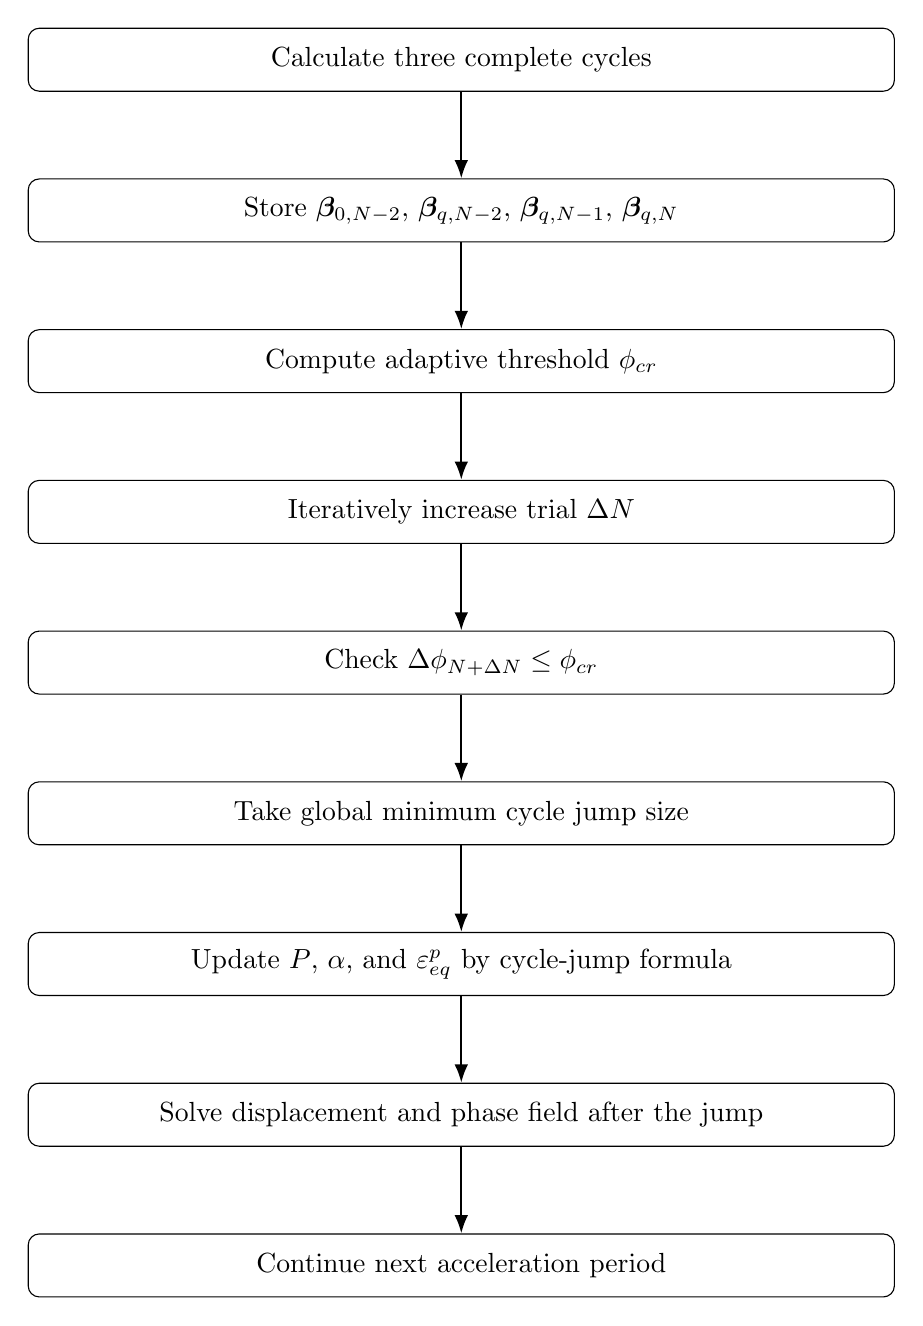
\begin{tikzpicture}[
    node distance=1.1cm,
    box/.style={rectangle, draw, rounded corners, align=center, minimum width=11cm, minimum height=0.8cm},
    arrow/.style={-{Latex}, thick}
]
\node[box] (a) {Calculate three complete cycles};
\node[box, below=of a] (b) {Store $\bm{\beta}_{0,N-2}$, $\bm{\beta}_{q,N-2}$, $\bm{\beta}_{q,N-1}$, $\bm{\beta}_{q,N}$};
\node[box, below=of b] (c) {Compute adaptive threshold $\phi_{cr}$};
\node[box, below=of c] (d) {Iteratively increase trial $\Delta N$};
\node[box, below=of d] (e) {Check $\Delta \phi_{N+\Delta N} \leq \phi_{cr}$};
\node[box, below=of e] (f) {Take global minimum cycle jump size};
\node[box, below=of f] (g) {Update $P$, $\alpha$, and $\varepsilon_{eq}^{p}$ by cycle-jump formula};
\node[box, below=of g] (h) {Solve displacement and phase field after the jump};
\node[box, below=of h] (i) {Continue next acceleration period};

\draw[arrow] (a) -- (b);
\draw[arrow] (b) -- (c);
\draw[arrow] (c) -- (d);
\draw[arrow] (d) -- (e);
\draw[arrow] (e) -- (f);
\draw[arrow] (f) -- (g);
\draw[arrow] (g) -- (h);
\draw[arrow] (h) -- (i);
\end{tikzpicture}
\caption{Flowchart of the adaptive explicit cycle-jump method in Li et al.}
\end{figure}

% ------------------------------------------------------------
\subsection{Important Figures to Study in Li et al.}

\begin{longtable}{p{0.18\textwidth}p{0.72\textwidth}}
\caption{Important figures in Li et al.} \\
\toprule
Figure & Why it is important \\
\midrule
\endfirsthead
\toprule
Figure & Why it is important \\
\midrule
\endhead

Fig. 1 & Schematic of explicit cycle jump. Shows how variables from several computed cycles are used to predict the state after a jump. \\

Fig. 2 & Evolution-rate curve. Helps understand why the change of $\bm{\beta}$ over $\Delta N$ is treated as an integral of the evolution rate. \\

Fig. 3 & Adaptive criterion illustration. Shows how $\Delta \phi_{N+\Delta N}$ and $\phi_{cr}$ control the jump size. \\

Fig. 4 & Loading waveform for accelerated examples. Important because the acceleration period consists of three real cycles plus a jump increment. \\

Fig. 5 & SENT geometry and boundary conditions. First main verification specimen. \\

Fig. 9 & Key elasto-plastic SENT result. Shows crack length, equivalent plastic strain, and crack path. Very important for understanding why $\varepsilon_{eq}^p$ is extrapolated. \\

Fig. 10 & Cycle jump size versus cycle number. Shows how $\Delta N$ changes automatically during crack growth. \\

Fig. 11 & Spatial distribution of cycle jump size and phase field. Very important: the crack-tip region controls the global jump size. \\

Fig. 14 & Different plastic constitutive models. Shows applicability to linear hardening and Armstrong--Frederick model. \\

Fig. 22 & Three-point bending result. Shows the method works beyond the simple SENT case. \\

Fig. 28 & Compact tension result and Paris-law comparison. Important for fracture-mechanics validation. \\

\bottomrule
\end{longtable}

% ------------------------------------------------------------
\subsection{What Problem Li et al. Solve}

Li et al. solve the problem of computationally expensive phase-field fatigue crack propagation simulations in elasto-plastic materials. The direct cycle-by-cycle approach is too slow because:

\begin{itemize}
    \item the phase-field crack requires fine mesh,
    \item crack growth needs many cycles,
    \item plasticity at the crack tip adds nonlinear constitutive cost,
    \item fatigue crack propagation life is not known in advance.
\end{itemize}

Their solution is an adaptive explicit cycle-jump method that predicts the evolution of selected crack-driving and plasticity variables, while automatically controlling the jump size using the phase-field evolution.

% ------------------------------------------------------------
\subsection{Key Takeaway from Li et al.}

The most important thesis lesson from Li et al. is:

\begin{quote}
For elasto-plastic fatigue crack propagation, cycle jumping must update not only fatigue/crack variables but also a plasticity-related variable, because crack-tip plasticity affects crack growth.
\end{quote}

% ============================================================
\newpage
\section{Paper 2: Cheng, Hu and Kirka (2022)}

\subsection{Full Reference}

Cheng, J., Hu, X., and Kirka, M. (2022). \textit{A cycle-jump acceleration method for the crystal plasticity simulation of high cycle fatigue of the metallic microstructure}. International Journal of Fatigue.

% ------------------------------------------------------------
\subsection{Main Idea}

Cheng, Hu and Kirka develop a cycle-jump acceleration method for crystal plasticity finite element simulations of high-cycle fatigue in metallic microstructures.

The key idea is:

\begin{quote}
Use crystal plasticity to simulate a few full cycles, extrapolate the internal state variables over many skipped cycles, then perform a re-equilibration step so that the finite element displacement and stress fields become consistent with the extrapolated internal variables.
\end{quote}

The method is implemented in Abaqus/Standard using user subroutines.

% ------------------------------------------------------------
\subsection{Why This Paper Matters}

This paper is very relevant for thesis work involving Abaqus and constitutive modeling because it is directly connected to:

\begin{itemize}
    \item metallic cyclic plasticity,
    \item microstructure-based finite element modeling,
    \item crystal plasticity internal variables,
    \item Abaqus/Standard implementation,
    \item UMAT and UEXTERNALDB style workflows,
    \item high-cycle fatigue acceleration.
\end{itemize}

Unlike Li et al., which focuses on phase-field crack propagation, Cheng et al. focus on cyclic plasticity inside a metallic microstructure before final fatigue failure.

% ------------------------------------------------------------
\subsection{Physical Model}

The model represents an ACMZ aluminium alloy microstructure obtained from EBSD data. The microstructure contains:

\begin{itemize}
    \item Al matrix grains,
    \item Cu-based grain-boundary particles,
    \item grain orientations from EBSD,
    \item finite element mesh representation of the microstructure.
\end{itemize}

The study uses a crystal plasticity finite element model to resolve local stress, strain, and slip evolution in the microstructure.

\begin{table}[H]
\centering
\caption{Physical model in Cheng et al.}
\begin{tabular}{lll}
\toprule
Feature & Description & Importance \\
\midrule
Material & ACMZ aluminium alloy & metallic microstructure \\
Microstructure source & EBSD image & real microstructure morphology \\
Matrix & Al grains & crystal plasticity behavior \\
Particles & Cu-based grain-boundary particles & elastic inclusions / stress concentrators \\
FE solver & Abaqus/Standard & implicit FE implementation \\
Element type & C3D8R & reduced-integration brick elements \\
\bottomrule
\end{tabular}
\end{table}

% ------------------------------------------------------------
\subsection{Crystal Plasticity Material Model}

The Al grains are modeled using a power-law crystal plasticity formulation. Grain-boundary particles are treated as elastic.

\subsubsection{Multiplicative Decomposition}

The total deformation gradient is decomposed into elastic and plastic parts:

\begin{equation}
\bm{F}
=
\bm{F}^e \bm{F}^p .
\end{equation}

Here:

\begin{itemize}
    \item $\bm{F}$ is the total deformation gradient,
    \item $\bm{F}^e$ is the elastic deformation gradient,
    \item $\bm{F}^p$ is the plastic deformation gradient.
\end{itemize}

\subsubsection{Plastic Velocity Gradient}

The plastic velocity gradient is written as a sum over slip systems:

\begin{equation}
\bm{L}^p
=
\dot{\bm{F}}^p(\bm{F}^p)^{-1}
=
\sum_{\alpha}
\dot{\gamma}^{\alpha}
\bm{s}^{\alpha}
\otimes
\bm{m}^{\alpha}.
\end{equation}

Here:

\begin{itemize}
    \item $\alpha$ is the slip-system index,
    \item $\dot{\gamma}^{\alpha}$ is the slip rate on slip system $\alpha$,
    \item $\bm{s}^{\alpha}$ is the slip direction,
    \item $\bm{m}^{\alpha}$ is the slip-plane normal.
\end{itemize}

\subsubsection{Stress Relation}

The Cauchy stress can be obtained from the elastic deformation and the second Piola--Kirchhoff stress. In crystal plasticity, the stress is computed from the elastic strain measure and the anisotropic elastic stiffness tensor.

A compact representation is:

\begin{equation}
\bm{S}
=
\mathbb{C}^e :
\bm{E}^e ,
\end{equation}

where:

\begin{itemize}
    \item $\bm{S}$ is the second Piola--Kirchhoff stress,
    \item $\mathbb{C}^e$ is the elastic stiffness tensor,
    \item $\bm{E}^e$ is the elastic Green strain.
\end{itemize}

The Cauchy stress follows from push-forward of the stress measure.

\subsubsection{Power-Law Slip Rule}

The slip rate is governed by a power-law relation:

\begin{equation}
\dot{\gamma}^{\alpha}
=
\dot{\gamma}_0
\left|
\frac{\tau^{\alpha}-\chi^{\alpha}}
{g^{\alpha}}
\right|^{1/m}
\text{sign}
(\tau^{\alpha}-\chi^{\alpha}) .
\end{equation}

Here:

\begin{itemize}
    \item $\dot{\gamma}_0$ is the reference slip rate,
    \item $\tau^{\alpha}$ is the resolved shear stress,
    \item $\chi^{\alpha}$ is the backstress on slip system $\alpha$,
    \item $g^{\alpha}$ is the slip resistance,
    \item $m$ is the strain-rate sensitivity parameter.
\end{itemize}

\subsubsection{Accumulated Slip}

The accumulated slip is:

\begin{equation}
\gamma
=
\int_0^t
\sum_{\alpha}
|\dot{\gamma}^{\alpha}|
\,d\xi .
\end{equation}

This is similar to an odometer for total slip activity in the crystal.

\subsubsection{Slip Resistance Hardening}

A saturation-type hardening law is used for the slip resistance:

\begin{equation}
g^{\alpha}
=
 g_0^{\alpha}
+
(g_s^{\alpha}-g_0^{\alpha})
\left[
1-
\exp
\left(
-\frac{h_0^{\alpha}\gamma}
{g_s^{\alpha}}
\right)
\right].
\end{equation}

Here:

\begin{itemize}
    \item $g_0^{\alpha}$ is the initial slip resistance,
    \item $g_s^{\alpha}$ is the saturation slip resistance,
    \item $h_0^{\alpha}$ is a hardening parameter,
    \item $\gamma$ is accumulated slip.
\end{itemize}

\subsubsection{Hall--Petch Grain-Size Dependence}

The initial slip resistance includes a Hall--Petch type relation:

\begin{equation}
g_0^{\alpha}
=
\bar{g}_0^{\alpha}
+
\frac{k}{\sqrt{d^{\alpha}}}.
\end{equation}

Here:

\begin{itemize}
    \item $\bar{g}_0^{\alpha}$ is the base initial slip resistance,
    \item $k$ is the Hall--Petch parameter,
    \item $d^{\alpha}$ is an equivalent grain size.
\end{itemize}

\subsubsection{Armstrong--Frederick Backstress Evolution}

The backstress evolves as:

\begin{equation}
\dot{\chi}^{\alpha}
=
 c\dot{\gamma}^{\alpha}
-
 d\chi^{\alpha}
|\dot{\gamma}^{\alpha}| .
\end{equation}

Here:

\begin{itemize}
    \item $c$ controls kinematic hardening,
    \item $d$ controls dynamic recovery,
    \item $\chi^{\alpha}$ shifts the slip response and contributes to cyclic hysteresis.
\end{itemize}

% ------------------------------------------------------------
\subsection{Cycle-Jump Internal Variables}

The cycle-jump method extrapolates the internal variable set:

\begin{equation}
\bm{S}
=
\left\{
\bm{F}^p,\gamma,\chi^{\alpha}
\right\}.
\end{equation}

To avoid confusion with stress, this document calls this set the internal state array:

\begin{equation}
\mathcal{S}
=
\left\{
\bm{F}^p,\gamma,\chi^{\alpha}
\right\}.
\end{equation}

Meaning:

\begin{table}[H]
\centering
\caption{Variables extrapolated in Cheng et al.}
\begin{tabular}{lll}
\toprule
Variable & Meaning & Why it is extrapolated \\
\midrule
$\bm{F}^p$ & plastic deformation gradient & stores permanent crystal plastic deformation \\
$\gamma$ & accumulated slip & measures accumulated slip activity \\
$\chi^{\alpha}$ & slip-system backstress & stores kinematic hardening memory \\
\bottomrule
\end{tabular}
\end{table}

% ------------------------------------------------------------
\subsection{Cycle-Jump Postulations}

The method relies on two assumptions:

\begin{enumerate}
    \item The internal variables evolve slowly and smoothly enough over high cycles that they can be extrapolated.
    \item If the extrapolated internal variables are accurate, the finite element displacement and stress field can be recovered by a re-equilibration step.
\end{enumerate}

This is very important for understanding the paper.

The method does not extrapolate displacement directly. Instead, it extrapolates internal variables and then lets Abaqus re-equilibrate the displacement and stress fields.

% ------------------------------------------------------------
\subsection{Taylor Expansion of Internal Variables}

The general Taylor expansion for an internal state variable at integration point $i$ is:

\begin{equation}
\mathcal{S}_{i}^{N+\Delta N}
=
\mathcal{S}_{i}^{N}
+
\Delta N
\left(\mathcal{S}_{i}\right)'
+
\frac{\Delta N^2}{2}
\left(\mathcal{S}_{i}\right)''
+
O(\Delta N^3).
\end{equation}

Here:

\begin{itemize}
    \item $N$ is the current cycle,
    \item $\Delta N$ is the number of cycles to skip,
    \item $\mathcal{S}_{i}^{N}$ is the internal state at integration point $i$ at cycle $N$,
    \item $(\mathcal{S}_{i})'$ is the first derivative with respect to cycle number,
    \item $(\mathcal{S}_{i})''$ is the second derivative with respect to cycle number.
\end{itemize}

The first derivative is estimated by a backward difference:

\begin{equation}
(\mathcal{S}_{i})'
\approx
\mathcal{S}_{i}^{N}
-
\mathcal{S}_{i}^{N-1}.
\end{equation}

The second derivative is estimated as:

\begin{equation}
(\mathcal{S}_{i})''
\approx
\mathcal{S}_{i}^{N}
-
2\mathcal{S}_{i}^{N-1}
+
\mathcal{S}_{i}^{N-2}.
\end{equation}

The paper uses a backward Eulerian linear approximation:

\begin{equation}
\mathcal{S}_{i}^{N+\Delta N}
=
\mathcal{S}_{i}^{N}
+
\Delta N
(\mathcal{S}_{i})' .
\end{equation}

% ------------------------------------------------------------
\subsection{Adaptive Jump Criterion}

The linear approximation is acceptable only if the second-order term is small. The paper imposes:

\begin{equation}
\frac{\Delta N^2}{2}
\left|
(\mathcal{S}_{i})''
\right|
\leq
\left|
\mathcal{S}_{i}^{N}
\right|\epsilon .
\end{equation}

Here $\epsilon$ is an accuracy-control parameter.

Solving for the allowable local jump gives:

\begin{equation}
\Delta N_i
\leq
\sqrt{
\frac{
2|\mathcal{S}_{i}^{N}|\epsilon
}
{
|(\mathcal{S}_{i})''|
}
}.
\end{equation}

The global jump size is the minimum over all integration points:

\begin{equation}
\Delta N
=
\min_i
\left\lfloor
\Delta N_i
\right\rfloor .
\end{equation}

An upper bound is also imposed:

\begin{equation}
\Delta N \leq \Delta N_{\max}.
\end{equation}

% ------------------------------------------------------------
\subsection{Re-Equilibration Step}

After the internal variables are extrapolated, the total deformation field is not automatically consistent with them. Therefore, the method performs a re-equilibration step.

The idea is:

\begin{quote}
Fix the extrapolated plastic/internal variables, apply a virtual zero-load or zero-displacement increment, and let the implicit FE solver find a displacement/stress field that satisfies equilibrium.
\end{quote}

This is why the method is naturally suited to Abaqus/Standard and implicit FE simulation.

% ------------------------------------------------------------
\subsection{Numerical Strategy in Abaqus}

The method is implemented using:

\begin{itemize}
    \item \texttt{UEXTERNALDB} to store and update global internal-variable arrays,
    \item \texttt{UMAT} to define the crystal plasticity constitutive response,
    \item \texttt{DLOAD} for load-controlled cyclic loading,
    \item \texttt{DISP} for displacement-controlled cyclic loading.
\end{itemize}

% ------------------------------------------------------------
\subsection{Cycle-Jump Algorithm}

\begin{figure}[H]
\centering
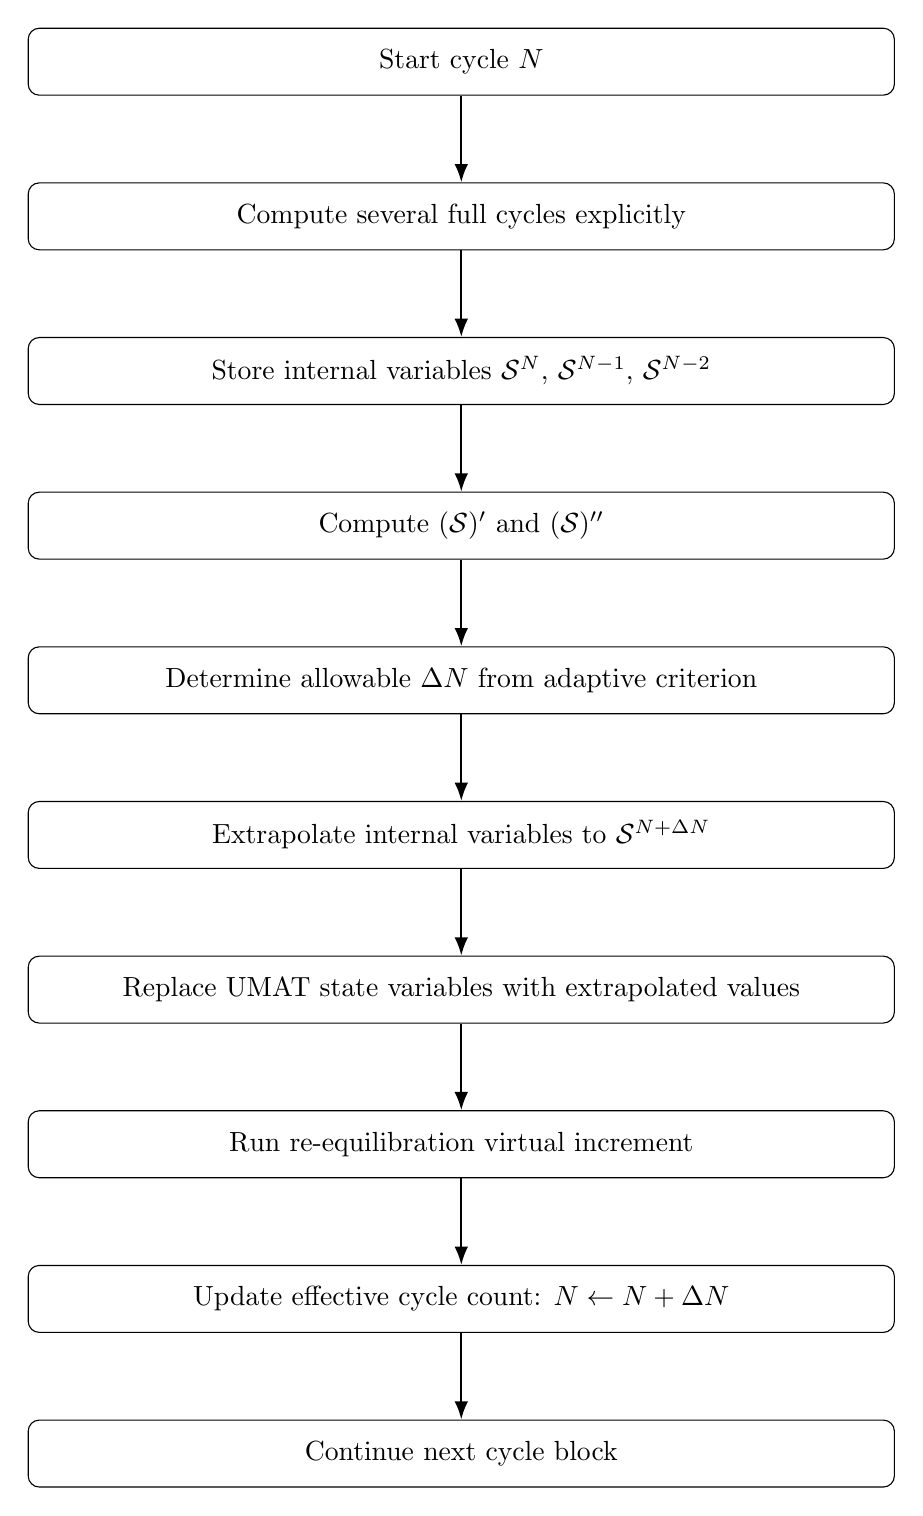
\begin{tikzpicture}[
    node distance=1.1cm,
    box/.style={rectangle, draw, rounded corners, align=center, minimum width=11cm, minimum height=0.85cm},
    arrow/.style={-{Latex}, thick}
]
\node[box] (a) {Start cycle $N$};
\node[box, below=of a] (b) {Compute several full cycles explicitly};
\node[box, below=of b] (c) {Store internal variables $\mathcal{S}^N$, $\mathcal{S}^{N-1}$, $\mathcal{S}^{N-2}$};
\node[box, below=of c] (d) {Compute $(\mathcal{S})'$ and $(\mathcal{S})''$};
\node[box, below=of d] (e) {Determine allowable $\Delta N$ from adaptive criterion};
\node[box, below=of e] (f) {Extrapolate internal variables to $\mathcal{S}^{N+\Delta N}$};
\node[box, below=of f] (g) {Replace UMAT state variables with extrapolated values};
\node[box, below=of g] (h) {Run re-equilibration virtual increment};
\node[box, below=of h] (i) {Update effective cycle count: $N \leftarrow N+\Delta N$};
\node[box, below=of i] (j) {Continue next cycle block};

\draw[arrow] (a) -- (b);
\draw[arrow] (b) -- (c);
\draw[arrow] (c) -- (d);
\draw[arrow] (d) -- (e);
\draw[arrow] (e) -- (f);
\draw[arrow] (f) -- (g);
\draw[arrow] (g) -- (h);
\draw[arrow] (h) -- (i);
\draw[arrow] (i) -- (j);
\end{tikzpicture}
\caption{Flowchart of the cycle-jump acceleration method in Cheng et al.}
\end{figure}

% ------------------------------------------------------------
\subsection{Important Figures to Study in Cheng et al.}

\begin{longtable}{p{0.18\textwidth}p{0.72\textwidth}}
\caption{Important figures in Cheng et al.} \\
\toprule
Figure & Why it is important \\
\midrule
\endfirsthead
\toprule
Figure & Why it is important \\
\midrule
\endhead

Fig. 1 & EBSD microstructure and converted FE mesh. This shows the physical microstructure being simulated. \\

Fig. 2 & Calibration of CPFE model against experimental tensile and hysteresis response. Important for material-model credibility. \\

Fig. 3 & Evolution of von Mises stress over cycles. Shows microstructural redistribution during cyclic loading. \\

Fig. 4 & Evolution of von Mises stress and accumulated slip along a line through the microstructure. Important for understanding why extrapolation is possible. \\

Fig. 5 & Known-state-variable cycle-jump validation. Shows that if state variables are known accurately, skipped-cycle displacement can be recovered. \\

Fig. 6 & Stress distribution comparison between reference and known-state-variable cycle-jump. Validates re-equilibration idea. \\

Fig. 7 & Main flowchart of the cycle-jump algorithm. This is the most important implementation figure. \\

Fig. 8 & Displacement comparison between conventional CPFE and cycle-jump method. Shows accuracy of the accelerated method. \\

Fig. 9 & Acceleration efficiency and jump distance. Shows how $\Delta N$ increases as evolution stabilizes. \\

Fig. 10 & von Mises stress error comparison. Important for accuracy assessment. \\

Fig. 11 & Accumulated slip at selected points. Shows internal-variable accuracy. \\

Fig. 13 & Higher load validation. Shows how larger plastic evolution reduces jump efficiency. \\

Fig. 15 & Negative $R$ ratio case. Important because reverse loading and kinematic hardening reduce acceleration efficiency. \\

Fig. 17 & Strain-controlled cyclic plasticity validation. Shows the method also works under displacement/strain control. \\

Fig. 19 & Elastic shakedown case. Important for seeing how rapid material-state changes affect acceleration efficiency. \\

Fig. 21 and Fig. 22 & Dislocation-density-based crystal plasticity validation. Shows applicability beyond the basic phenomenological CP model. \\

\bottomrule
\end{longtable}

% ------------------------------------------------------------
\subsection{What Problem Cheng et al. Solve}

Cheng et al. solve the problem of computationally expensive crystal plasticity finite element simulations for high-cycle fatigue.

A direct cycle-by-cycle CPFE simulation is too expensive because:

\begin{itemize}
    \item every loading and unloading cycle needs multiple increments,
    \item every integration point has many crystal plasticity state variables,
    \item microstructure-level stress redistribution evolves over many cycles,
    \item high-cycle fatigue may require thousands to millions of effective cycles.
\end{itemize}

Their solution is to extrapolate internal variables and use re-equilibration to recover consistent displacement and stress fields.

% ------------------------------------------------------------
\subsection{Key Takeaway from Cheng et al.}

The most important thesis lesson from Cheng et al. is:

\begin{quote}
For crystal plasticity fatigue, the cycle-jump method should extrapolate internal state variables, not simply external response quantities. After extrapolation, an implicit re-equilibration step is required to make the displacement and stress fields consistent with the jumped material state.
\end{quote}

% ============================================================
\newpage
\section{Comparison of the Two Papers}

\begin{longtable}{p{0.26\textwidth}p{0.34\textwidth}p{0.34\textwidth}}
\caption{Comparison of Li et al. and Cheng et al.} \\
\toprule
Aspect & Li et al. (2025) & Cheng, Hu \& Kirka (2022) \\
\midrule
\endfirsthead
\toprule
Aspect & Li et al. (2025) & Cheng, Hu \& Kirka (2022) \\
\midrule
\endhead

Main problem &
Accelerating elasto-plastic phase-field fatigue crack propagation. &
Accelerating high-cycle crystal plasticity simulation of metallic microstructures. \\

Physical model &
Cracked elasto-plastic continuum with phase-field fracture. &
Polycrystalline metallic microstructure from EBSD. \\

Main damage/crack variable &
Phase field $\phi$. &
No phase field; fatigue is related to cyclic plasticity and microstructural state evolution. \\

Material model &
J2 plasticity with linear hardening, power-law hardening, and Armstrong--Frederick cyclic model. &
Crystal plasticity with slip resistance, accumulated slip, and backstress. \\

Variables extrapolated &
$P$, $\alpha$, $\varepsilon_{eq}^p$. &
$\bm{F}^p$, accumulated slip $\gamma$, backstress $\chi^{\alpha}$. \\

Jump-size control &
Adaptive criterion based on phase-field evolution. &
Adaptive criterion based on linearity of internal-variable evolution. \\

Post-jump strategy &
Update selected variables, then solve displacement and phase-field equations. &
Extrapolate internal variables, then perform re-equilibration in Abaqus/Standard. \\

Abaqus implementation &
UEL for displacement/phase field, UMAT/CPE4 layer for post-processing. &
UMAT, UEXTERNALDB, DLOAD, DISP. \\

Most important figure &
Fig. 11: jump-size distribution and phase field. &
Fig. 7: cycle-jump algorithm flowchart. \\

Main thesis relevance &
Useful for future phase-field fatigue crack propagation and elasto-plastic crack-tip plasticity. &
Useful for future UMAT/cycle-jump implementation in cyclic plasticity. \\

\bottomrule
\end{longtable}

% ============================================================
\section{Common Cycle-Jump Logic}

Both papers follow the same broad idea:

\begin{enumerate}
    \item compute a few real cycles,
    \item identify slow evolution of important variables,
    \item estimate derivatives with respect to cycle number,
    \item choose a safe jump size,
    \item extrapolate selected variables,
    \item recover equilibrium or continue field solution,
    \item repeat.
\end{enumerate}

The key difference is the choice of variables.

Li et al. choose variables linked to crack driving force and plastic crack-tip accumulation:

\[
\bm{\beta} = [P,\alpha,\varepsilon_{eq}^p].
\]

Cheng et al. choose crystal plasticity internal variables:

\[
\mathcal{S}
=
\{\bm{F}^p,\gamma,\chi^{\alpha}\}.
\]

% ============================================================
\section{What This Means for My Thesis Direction}

The Abaqus built-in cyclic plasticity study is the correct preparation step before implementation. The reason is that both cycle-jump papers depend on understanding internal variables and cyclic evolution.

For future thesis work, the following path is reasonable:

\begin{enumerate}
    \item first understand Abaqus built-in cyclic plasticity models,
    \item then understand what internal variables evolve cycle by cycle,
    \item then study how cycle-jump methods extrapolate those internal variables,
    \item only after that consider UMAT/cycle-jump implementation.
\end{enumerate}

The present Abaqus study with linear kinematic, multilinear kinematic, and combined hardening is therefore useful because it gives practical understanding of:

\begin{itemize}
    \item hysteresis loops,
    \item PEEQ accumulation,
    \item cyclic hardening behavior,
    \item ratcheting-style response,
    \item post-processing of cyclic simulations.
\end{itemize}

% ============================================================
\section{Short Meeting Summary}

Li et al. (2025) propose an adaptive explicit cycle-jump method for elasto-plastic phase-field fatigue crack propagation. Their method extrapolates the history field $P$, fatigue history variable $\alpha$, and equivalent plastic strain $\varepsilon_{eq}^p$, while adapting the jump size based on phase-field evolution. This makes the method suitable for crack growth problems where crack-tip plasticity affects fatigue propagation.

Cheng, Hu and Kirka (2022) propose a cycle-jump acceleration method for crystal plasticity finite element simulations of high-cycle fatigue. Their method extrapolates crystal plasticity internal variables such as plastic deformation gradient, accumulated slip, and backstress. After each jump, a re-equilibration step in Abaqus/Standard recovers the consistent displacement and stress fields.

Together, the two papers show that cycle jumping is not simply skipping cycles. It is a controlled extrapolation of physically meaningful internal variables, combined with an error-control or adaptivity rule. This is directly relevant for future fatigue and UMAT work, but it requires strong understanding of the base cyclic plasticity model first.

% ============================================================
\section*{References}

\begin{enumerate}
    \item J. Li, Y. Hu, N. Ao, H. Miao, X. Zhang, G. Kang, and Q. Kan, ``An adaptive cycle jump method for elasto-plastic phase field modeling addressing fatigue crack propagation,'' \textit{Computer Methods in Applied Mechanics and Engineering}, vol. 442, 118074, 2025. DOI: \href{https://doi.org/10.1016/j.cma.2025.118074}{10.1016/j.cma.2025.118074}.
    \item J. Cheng, X. Hu, and M. Kirka, ``A cycle-jump acceleration method for the crystal plasticity simulation of high cycle fatigue of the metallic microstructure,'' \textit{International Journal of Fatigue}, 2022.
\end{enumerate}

\end{document}
